\documentclass[handout,nooutcomes]{ximera}

\usepackage{booktabs}
%% handout
%% space
%% newpage
%% numbers
%% nooutcomes


\renewcommand{\outcome}[1]{\marginpar{\null\vspace{2ex}\scriptsize\framebox{\parbox{0.75in}{\begin{raggedright}P\arabic{problem} Outcome: #1\end{raggedright}}}}}

\newcommand{\RR}{\mathbb R}
\renewcommand{\d}{\,d}
\newcommand{\dd}[2][]{\frac{d #1}{d #2}}
\renewcommand{\l}{\ell}
\newcommand{\ddx}{\frac{d}{dx}}
\everymath{\displaystyle}
\newcommand{\dfn}{\textbf}
\newcommand{\eval}[1]{\bigg[ #1 \bigg]}


\title{Breakout Session 3: Definitions of Limits}  

\begin{document}
\begin{abstract}
 \textbf{A look back:} In the previous (January 14, 2016) Breakout Session you discovered how we formulate instantaneous rate of change using limits, and practiced computing instantaneous velocity by using a graph, table of values, or algebraic manipulation.

 \textbf{Overview:} In today's (January 19, 2016) Breakout Session you will start investigating the notion of a limit more closely.
 The limit of a function is \emph{the} fundamental mathematical concept we will use to formulate instantaneous rate of change and accumulation.

  \textbf{A look ahead:} In the next (January 21, 2016) Breakout Session you will investigate how to compute limits, primarily using pen and paper, by ``reshaping harder limits into easier limits''.
\end{abstract}
\maketitle

\section{Learning Outcomes}
\label{section:learning-outcomes}
The following outcomes are \emph{not an exhaustive} list of the skills you will need to develop and integrate for demonstration on quizzes and exams.
This list is meant to be a starting point for conversation (with your Lecturer, Breakout Session Instructor, and fellow learners) for organizing your knowledge and monitoring the development of your skills.
\begin{itemize}
  \item 
    Find limits from a graph (or state that the limit does not exist).
  \item 
    Estimate limits using nearby values.
  \item 
    Define a one-sided limit.
  \item
    Distinguish between limit values and function values.
  \item 
    Identify the points where a limit does not exist and explain why.
\end{itemize}
\newpage
\section{Interpreting Limits}
\label{section:interpreting-limits}

\begin{problem}
  \label{problem:conceptual-check-on-limit-definition}
  \mbox{}
  \begin{itemize}
    \item[(a)]
      \textbf{True or False:}
      To find $\lim_{x \to 2} f(x)$, it's enough to know the values of $f(2.1)$, $f(2.01)$, $f(2.001)$, and so on.

    \item[(b)]
      \textbf{True or False:}
       If we know the value of $f(2)$, then we know the value of $\lim_{x \to 2} f(x)$.
  \end{itemize}
\end{problem}

\begin{problem}
  \label{problem:finding-limits-via-graphs}
  Use the graphs and the given definitions of the following two functions to answer the questions below.
  \begin{image}
    \hspace*{-5em}
    \includegraphics{Images/"Graph of rational function".png}
    \hspace*{3em}
        \includegraphics{Images/"Graph of linear function".png}
  \end{image}
  \begin{itemize}
    \item[(a)]
      Find the domain of $f$ and the domain of $g$.

    \item[(b)]
      Is $f = g$?
      (Why or why not?)

    \item[(c)]
      Looking at the graphs, find $\lim_{x \to 1} f(x)$ and $\lim_{x \to 1} g(x)$.
  \end{itemize}
\end{problem}

\begin{problem}
  \label{problem:reading-properties-of-function-from-graph}
  The graph of a function $f$ is given below.
  Use this graph to answer the following questions.
  \begin{image}
    \includegraphics[scale = 0.3]{Images/"Piecewise defined function".png}
  \end{image}
  \begin{itemize}
    \item[(I)]
        Find the domain of $f$.

    \item[(II)]
        Find the range of $f$.

    \item[(III)]
      Find the following values.
      \begin{itemize}
        \item[(a)]
          $\displaystyle \lim_{x \to -2} f(x) = $
        \item[(b)]
          $f(-2) = $
        \item[(c)]
          $f(-5) = $
        \item[(d)]
          $\displaystyle \lim_{x \to 0^+} f(x) = $
        \item[(e)]
          $\displaystyle \lim_{x \to 0} f(x) = $
      \end{itemize}
  \end{itemize}

\end{problem}

\section{Graphing functions}
\label{section:graphing-functions}

\begin{problem}
  \label{problem:sketch-a-graph-using-limits}
   Sketch the graph of a function that satisfies all of the given properties.
  (You \emph{do not} need to find a formula for the function.)
  \begin{center}
    \begin{tabular}[c]{llll}
      \toprule
      & & \hspace{-5em}Required Properties\\
      \midrule
      $f(3) = -2$ & $f(5) = 6$ & $\displaystyle \lim_{x \to 5^-} f(x) = -1$ & $\displaystyle \lim_{x \to 5^+} f(x) = 4$ \\
      $\displaystyle \lim_{x \to 3} f(x) = 7$ & $\displaystyle \lim_{x \to -5^-} f(x) = 3$ & $\displaystyle \lim_{x \to -2^+} f(x) = 0$ & $\displaystyle \lim_{x \to 1^+} f(x) = 5$\\
      \bottomrule
    \end{tabular}
  \end{center}
\end{problem}

\section{Extra Problem for Personal Practice}
\label{section:extra-problems}
\begin{problem}
  \textbf{True or False}: Give an explanation or counterexample.
  Assume $a$ and $L$ are finite numbers.
  \begin{itemize}
    \item[(a)]
      If $ \lim_{x \to a} f(x) = L$, then $f(a) = L$.
    \item[(b)]
      If $  \lim_{x \to a^-} f(x) = L$, then $  \lim_{x \to a^+} f(x) = L $.
    \item[(c)]
      If $ \lim_{x \to a} f(x) = L $ and $  \lim_{x \to a} g(x) = L $, then $f(a) = g(a)$.
    \item[(d)]
       $ \lim_{x \to a} \frac{f(x)}{g(x)} $ does not exist if $g(a) = 0$.
  \end{itemize}
\end{problem}


% \section*{Warm up:} 

% 	\begin{enumerate}[label=(\alph*)]
	
% 	\item  True or False: To find $\lim_{x \to 2} f(x)$, it's enough to know $f(2.1)$, $f(2.01)$, $f(2.001)$, etc.
% 	\begin{freeResponse}
% 	 False.  These values will only help us make a guess at $\lim_{x \to 2^+} f(x)$, the right hand limit of $f(x)$.  To determine $\lim_{x \to 2} f(x)$, we also need to know $\lim_{x \to 2^-} f(x)$ which we cannot determine from the above values.  For example, consider the function
% 	 	\begin{image}
% 	 	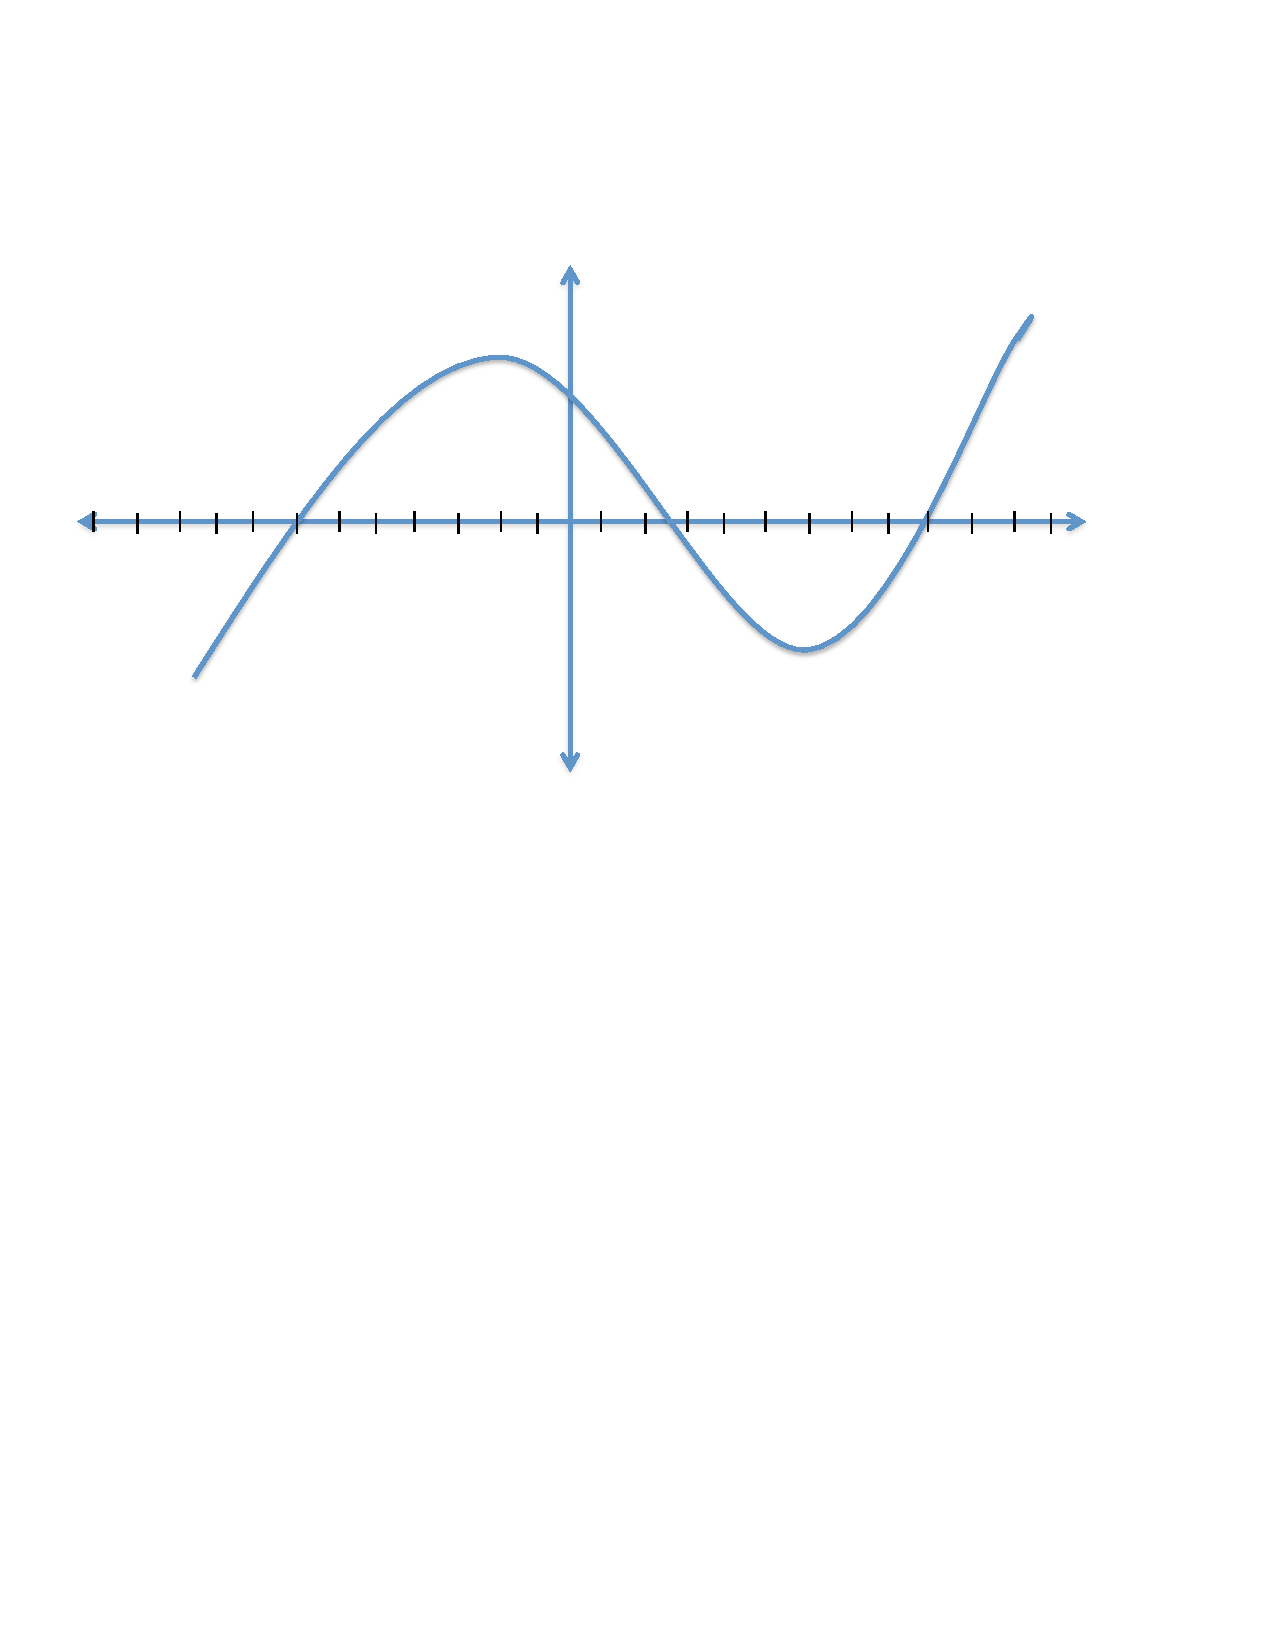
\includegraphics[trim= 70 570 300 165]{Figure2.pdf}
% 	 	\end{image}
	 	
% 	Looking at the graph of this function below, we can see that $\lim_{x \to 2^+} f(x) = 1$ and $\lim_{x \to 2^-} f(x) = -1$.  Thus, since $\lim_{x \to 2^+} f(x) \neq \lim_{x \to 2^-} f(x)$, $\lim_{x \to 2} f(x)$ does not exist.
	
% 		\begin{image}
% 		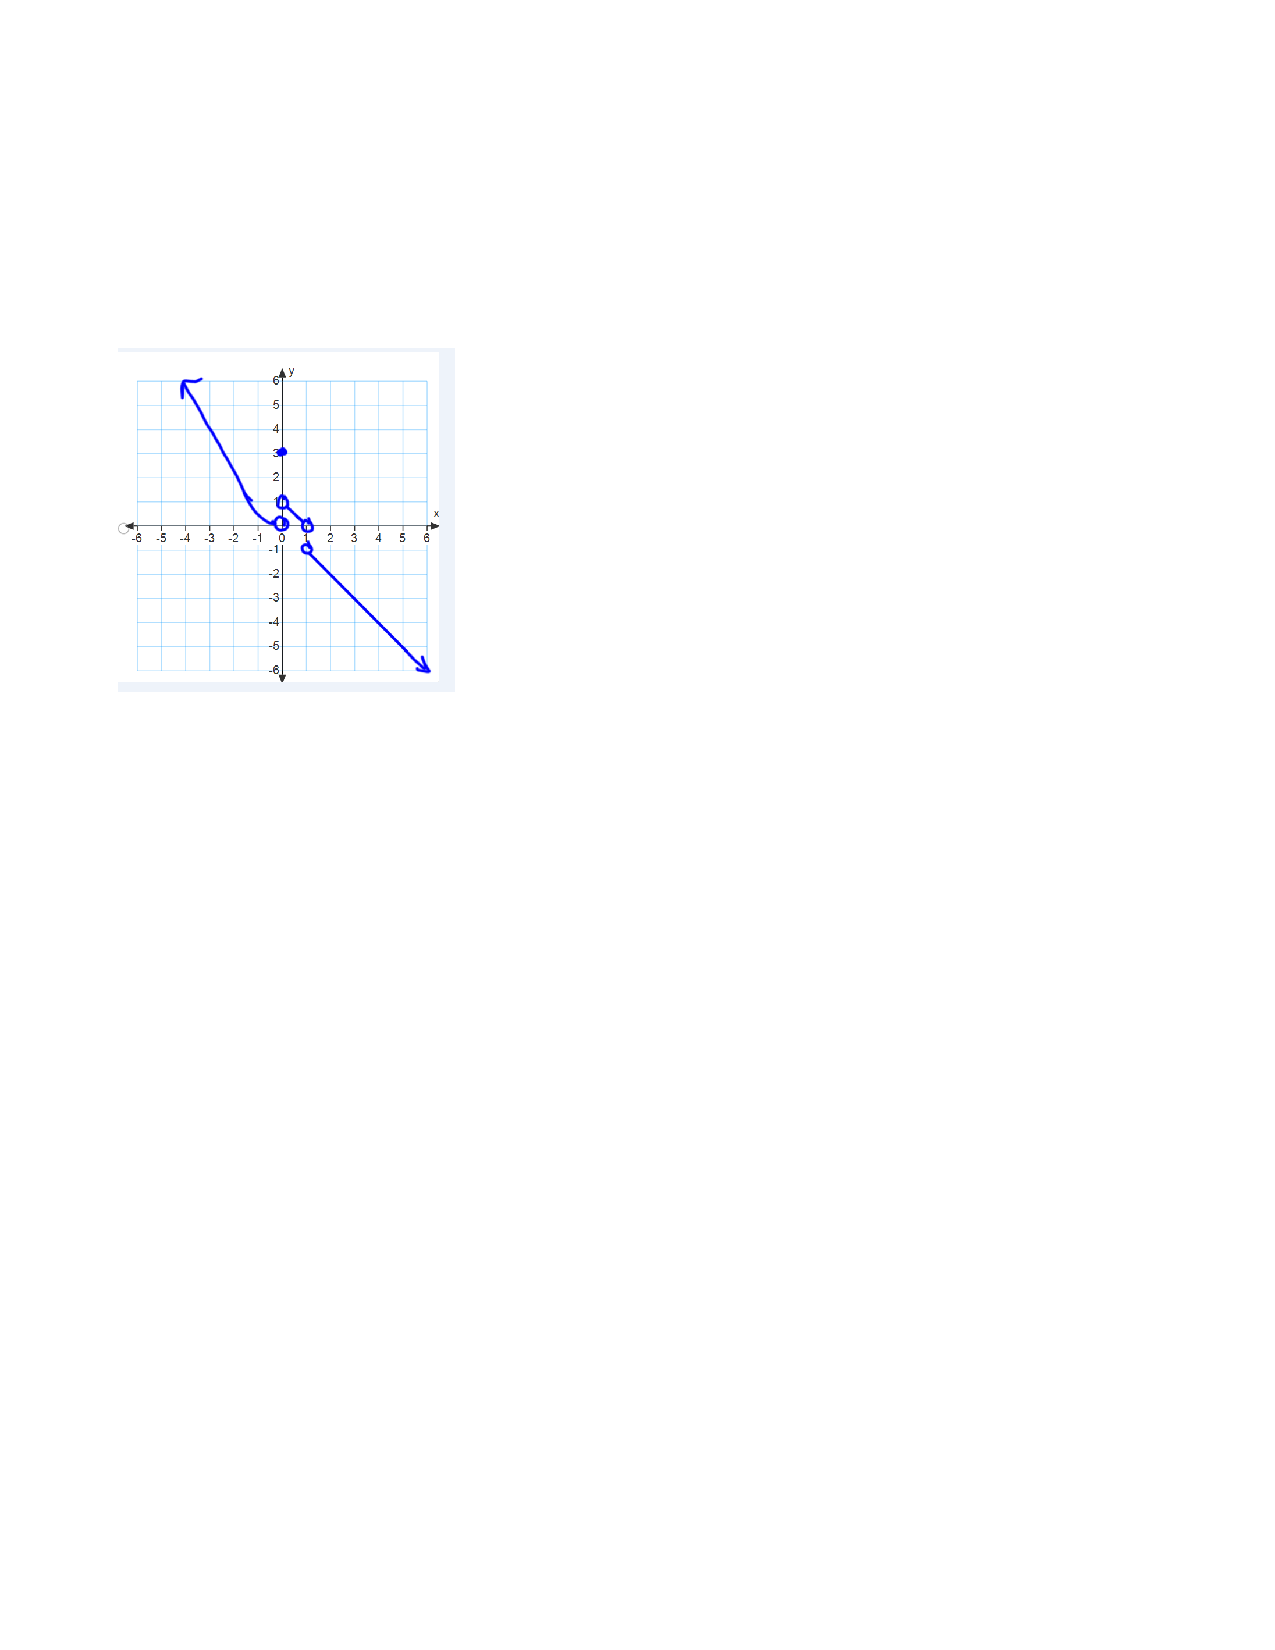
\includegraphics[trim= 70 470 250 160]{Figure3.pdf}
% 		\end{image}
% 	\end{freeResponse}
	
	
	
% 	\item  True or False: If we know $f(2)$, then we know $\lim_{x \to 2} f(x)$.
% 		\begin{freeResponse}
% 		False.  In the above example, we have that $f(2) = 0$, however $\lim_{x \to 2} f(x)$ does not exist.
% 		\end{freeResponse}
% 	\end{enumerate}



% \section*{Group work:}

% %Problem 1	
% \begin{problem}
% Given the graph of the function, estimate $\lim_{x \to 1} \frac{x^2 - 1}{x - 1} $.  Then estimate $\lim_{x \to 1} \frac{x^2 - 1}{x - 1} $ by creating a table of values.
	
% 	\begin{image}
% 	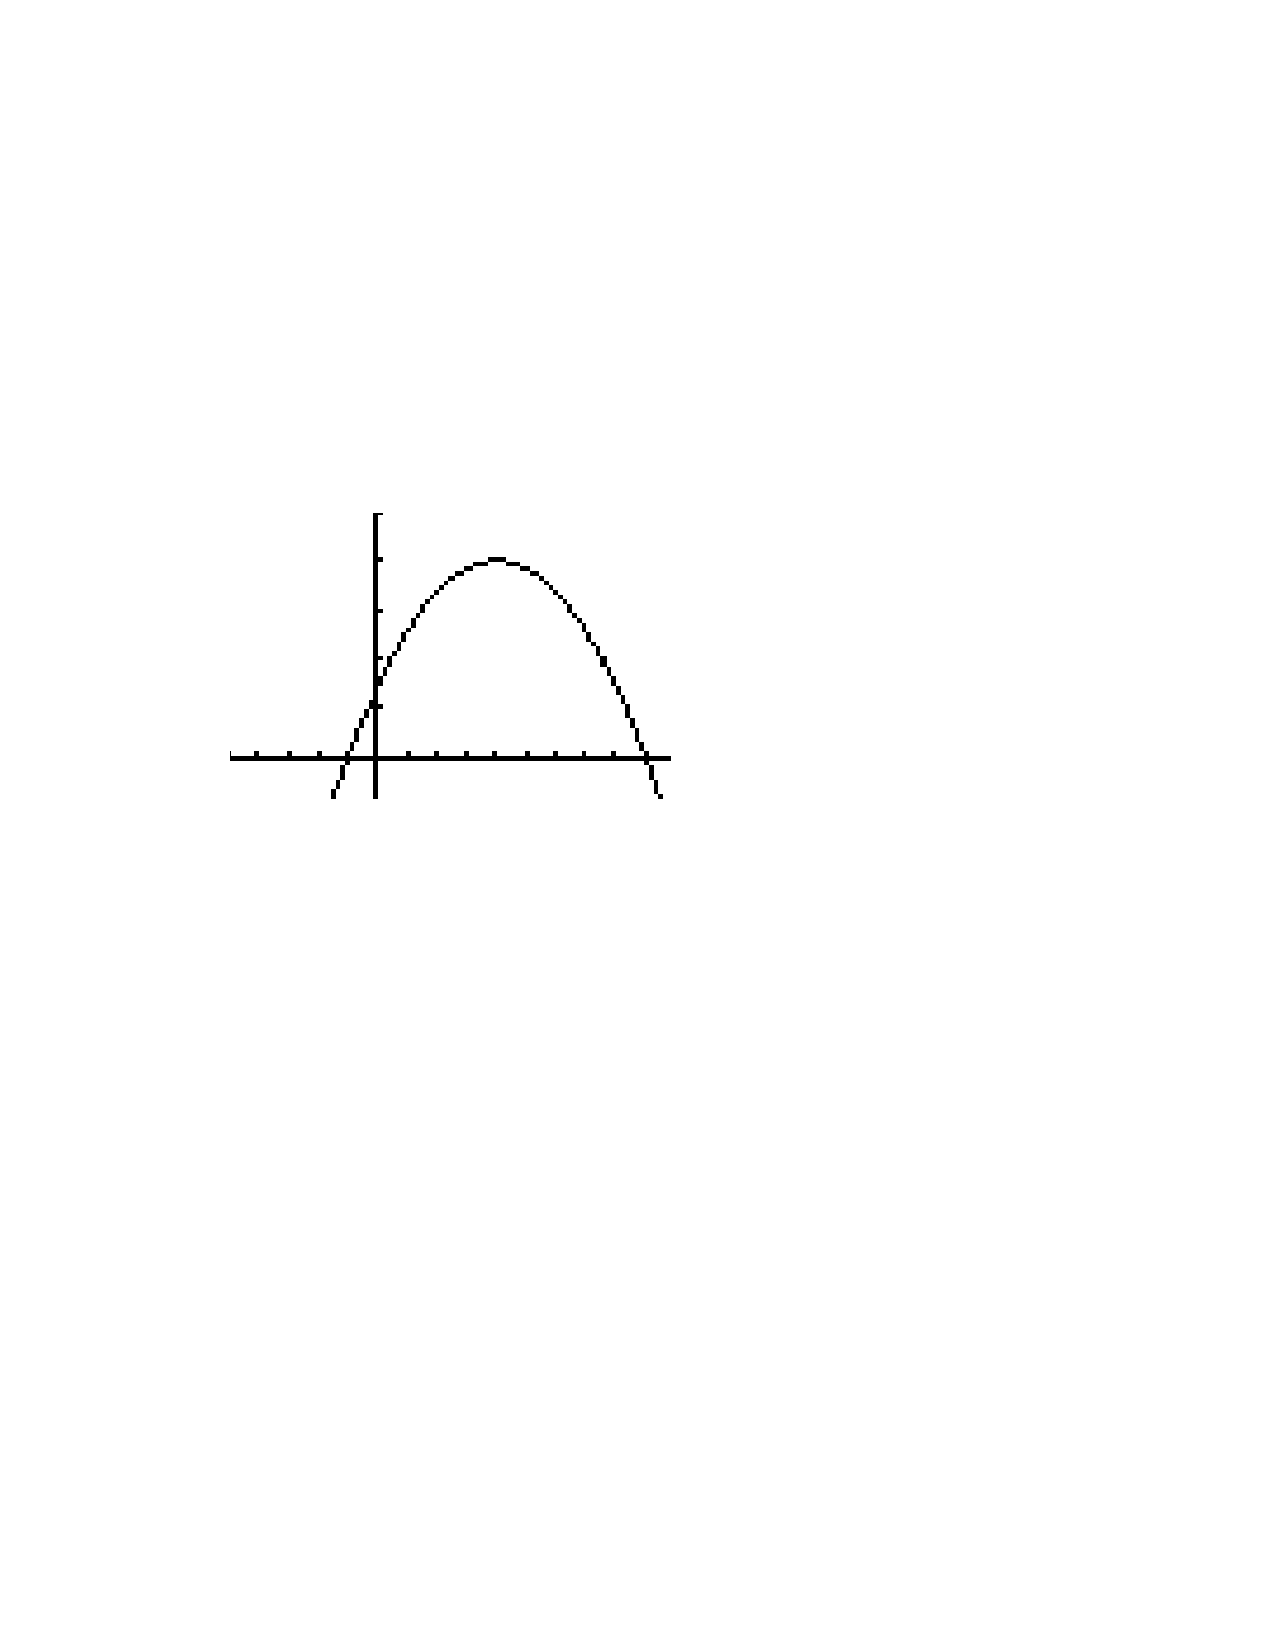
\includegraphics[trim= 50 470 300 135]{Figure1.pdf}
% 	\end{image}
	
% 	\begin{freeResponse}
% 	From the graph and table of values, it appears as though $\lim_{x \to 1} f(x) = 2$.
	
% 	\begin{tabular}{|l|l|}
% 	\hline
% 	\hspace{2mm} $x$ & \hspace{4mm} $f(x)$  \\
% 	\hline
% 	.9 & $ \frac{{{.9}^{2}}-1}{.9-1}=1.9  $  \\
% 	\hline
% 	.99 & $ \frac{{{.99}^{2}}-1}{.99-1}=1.99 $  \\
% 	\hline
% 	.999 & $ \frac{{{.999}^{2}}-1}{.999-1}=1.999 $  \\
% 	\hline
% 	1.1 & $ \frac{{{1.1}^{2}}-1}{1.1-1}=2.1 $  \\
% 	\hline
% 	1.01 & $ \frac{{{1.01}^{2}}-1}{1.01-1}=2.01 $  \\
% 	\hline
% 	1.001 & $ \frac{{{1.001}^{2}}-1}{1.001-1}=2.001 $  \\
% 	\hline
% 	\end{tabular}
	
% 	\end{freeResponse}
	
% \end{problem}
			
			
			

% %Problem 2
% \begin{problem}
% Sketch the graph of a function with the given properties.  You need not find a formula for the function.
% 	$$ f(3) = -2 , f(5) = 6 , \lim_{x \to 5^-} f(x) = -1 ,   \lim_{x \to 5^+} f(x) = 4 ,  \lim_{x \to 3} f(x) = 7 $$
% 	$$  \lim_{x \to -2^-} f(x) = 3 ,  \lim_{x \to -2^+} f(x) = 0 ,  \lim_{x \to 1^+} f(x) = 5  $$
% 	\begin{freeResponse}
% 	While there are many correct solutions to this problem, one example can be seen below.
	
% 		\begin{image}
% 		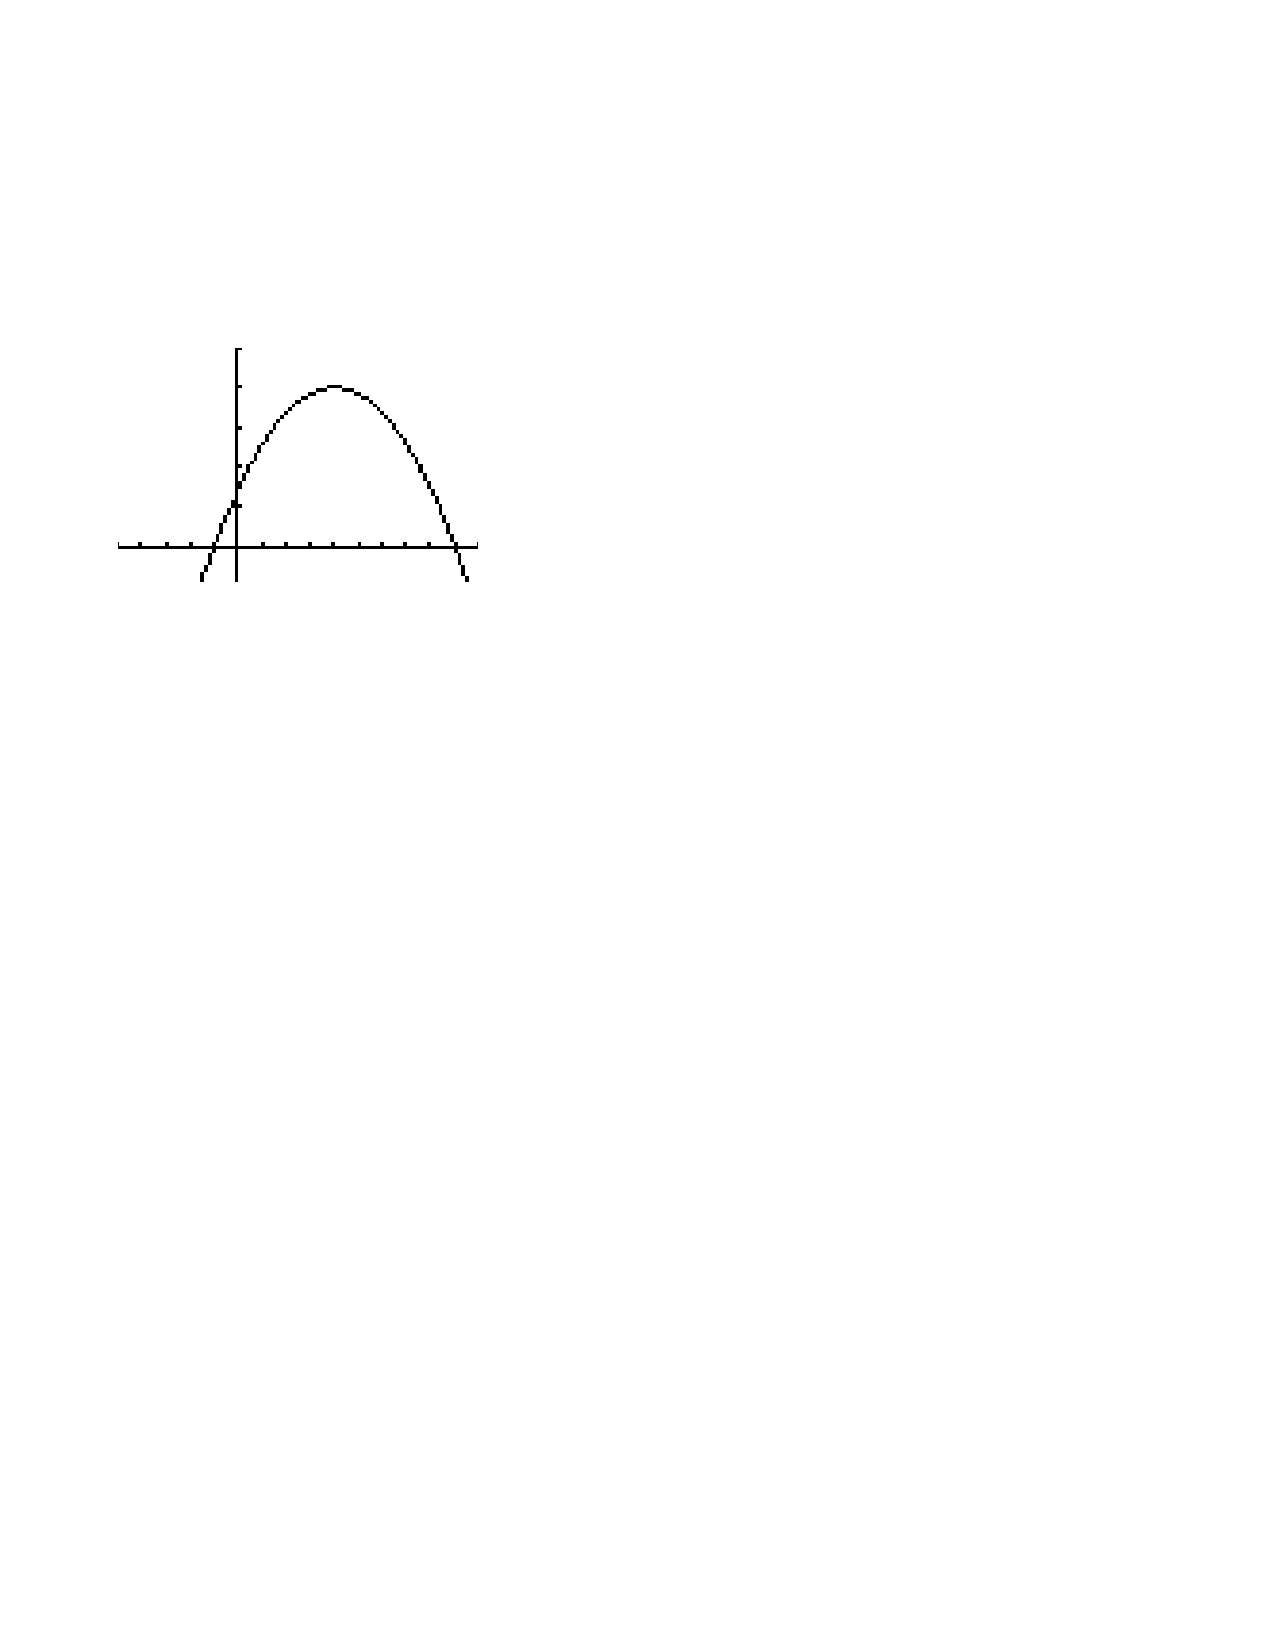
\includegraphics[trim= 70 470 250 160]{Figure4.pdf}
% 		\end{image}
% 	\end{freeResponse}
% \end{problem}
	
	
	
	

% %Problem 3	
% \begin{problem}
% True/False:  Give an explanation or counterexample.  Assume $a$ and $L$ are finite numbers.
	
% 			\begin{enumerate}
			
% 			%part a
% 			\item  If $ \lim_{x \to a} f(x) = L$, then $f(a) = L$.
% 			\begin{freeResponse}
% 			False.  In the graph below $ \lim_{x \to 1} f(x) = 2 $, but $f(1)$ does not exist.
			
% 				\begin{image}
% 				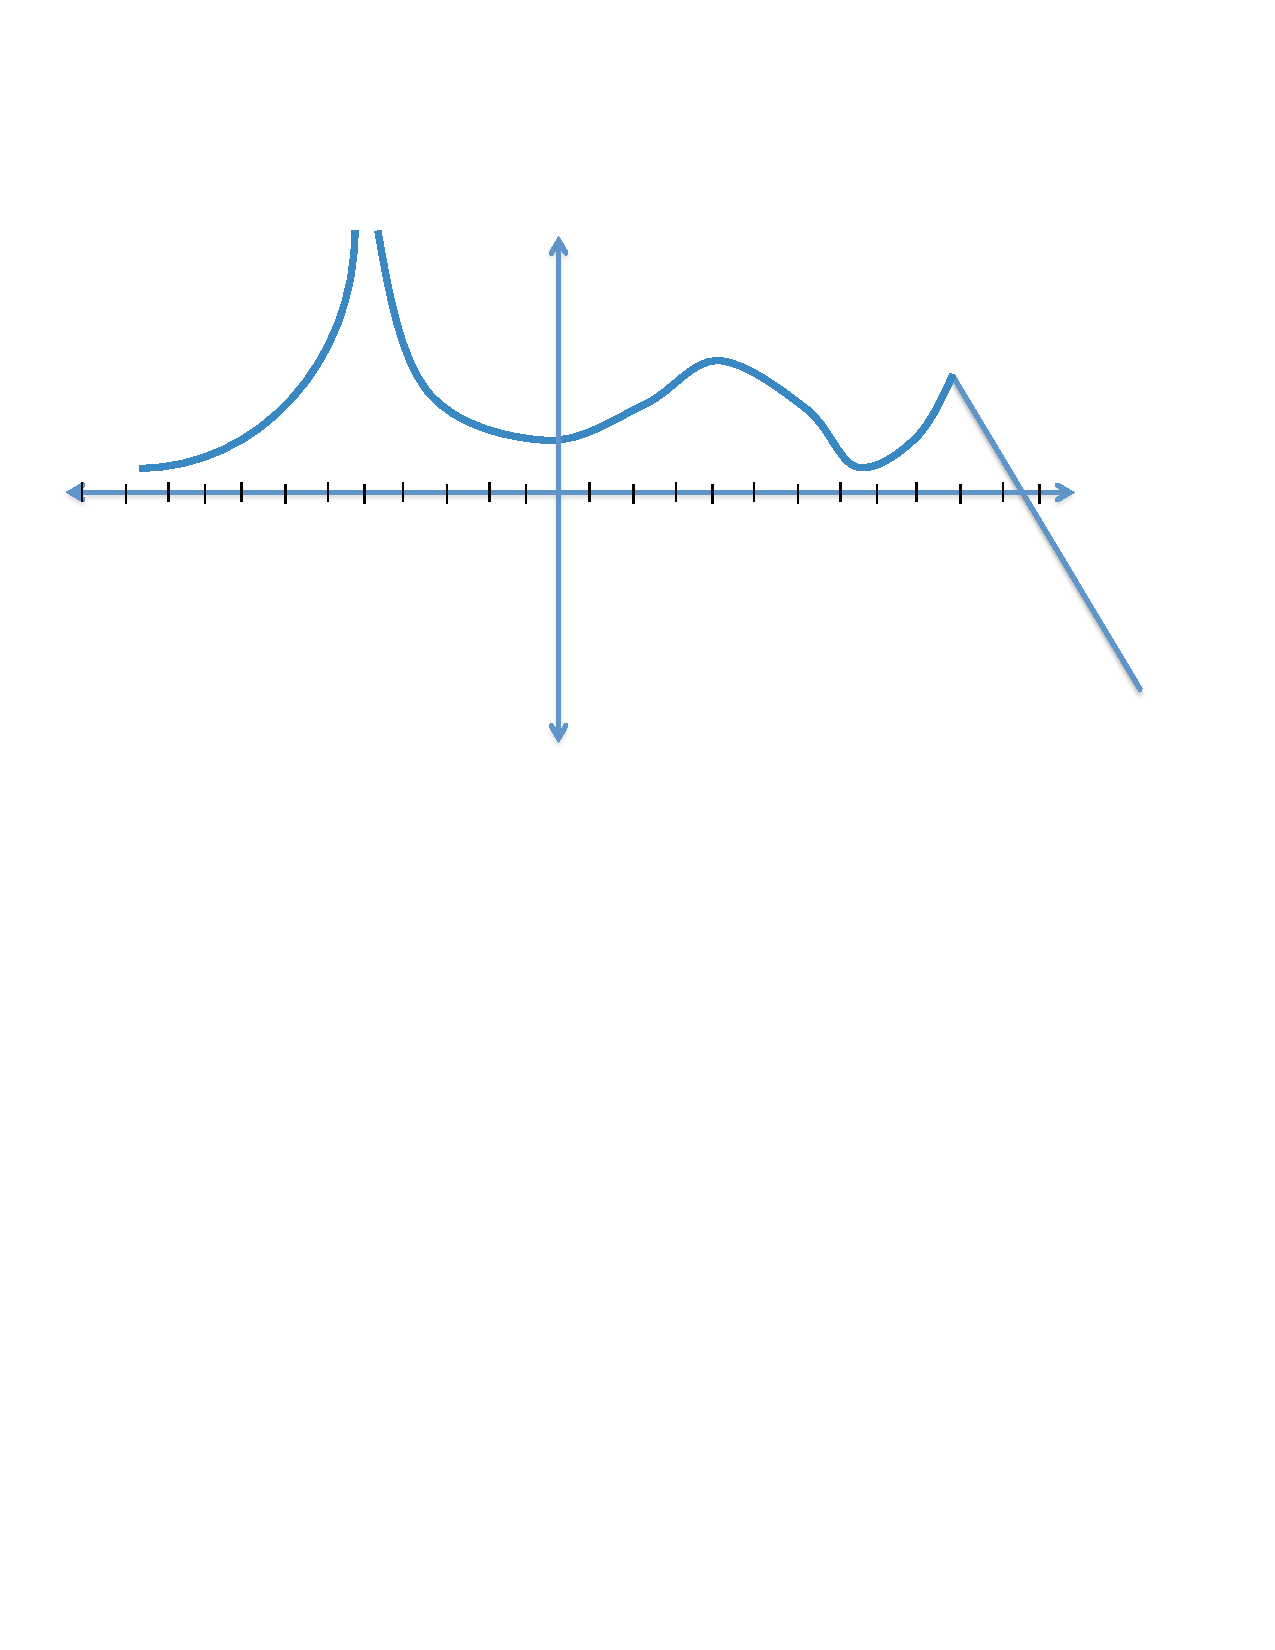
\includegraphics[trim= 70 470 250 160]{Figure5.pdf}
% 				\end{image}
% 			\end{freeResponse}
			
			
			
% 			%part b
% 			\item  If $  \lim_{x \to a^-} f(x) = L$, then $  \lim_{x \to a^+} f(x) = L $.
% 			\begin{freeResponse}
% 			False.  In the graph below $ \lim_{x \to 1^-} f(x) = 5$ but $ \lim_{x \to 1^+} f(x) = 6$.
			
% 				\begin{image}
% 				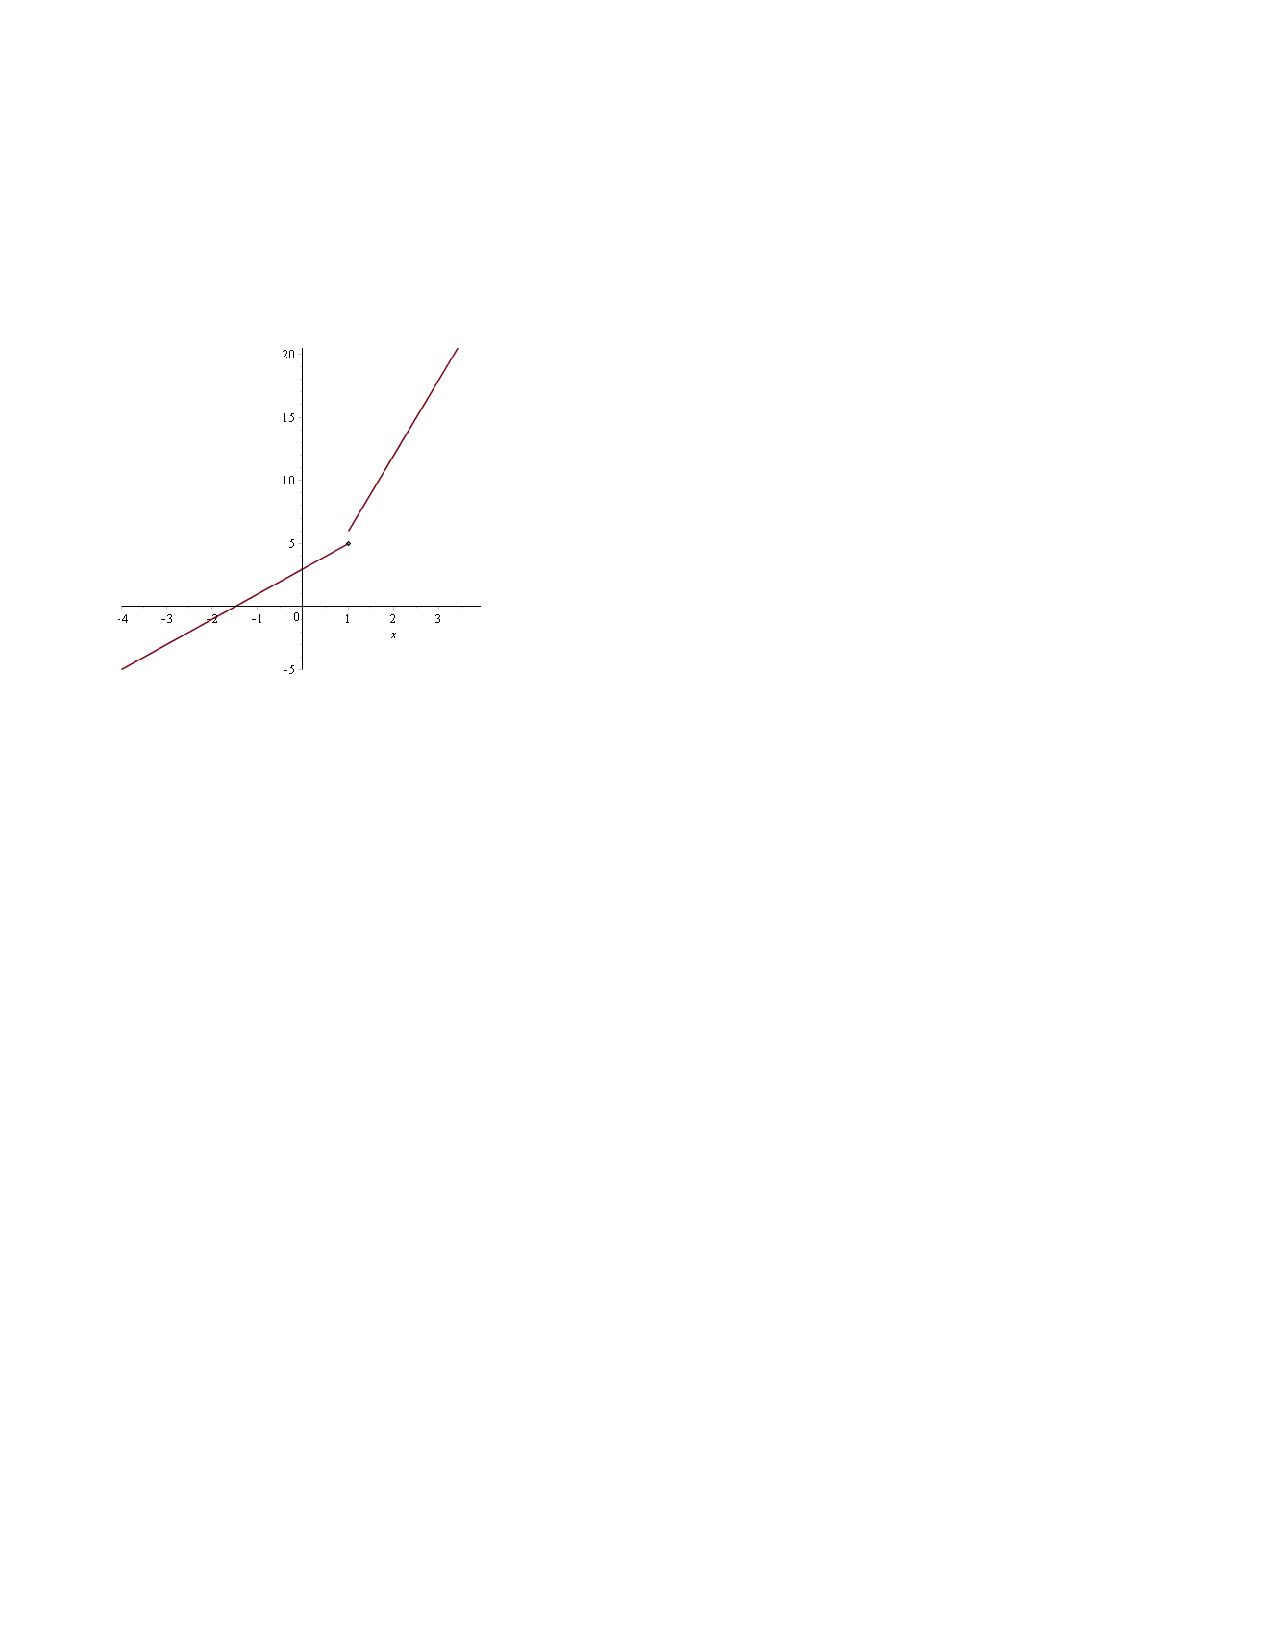
\includegraphics[trim= 70 470 250 160]{Figure6.pdf}
% 				\end{image}
% 			\end{freeResponse}
			
			
			
% 			%part c
% 			\item  If $ \lim_{x \to a} f(x) = L $ and $  \lim_{x \to a} g(x) = L $, then $f(a) = g(a)$.
% 			\begin{freeResponse}
% 			 False.  If we let 
			 
% 			 	\begin{image}
% 			 	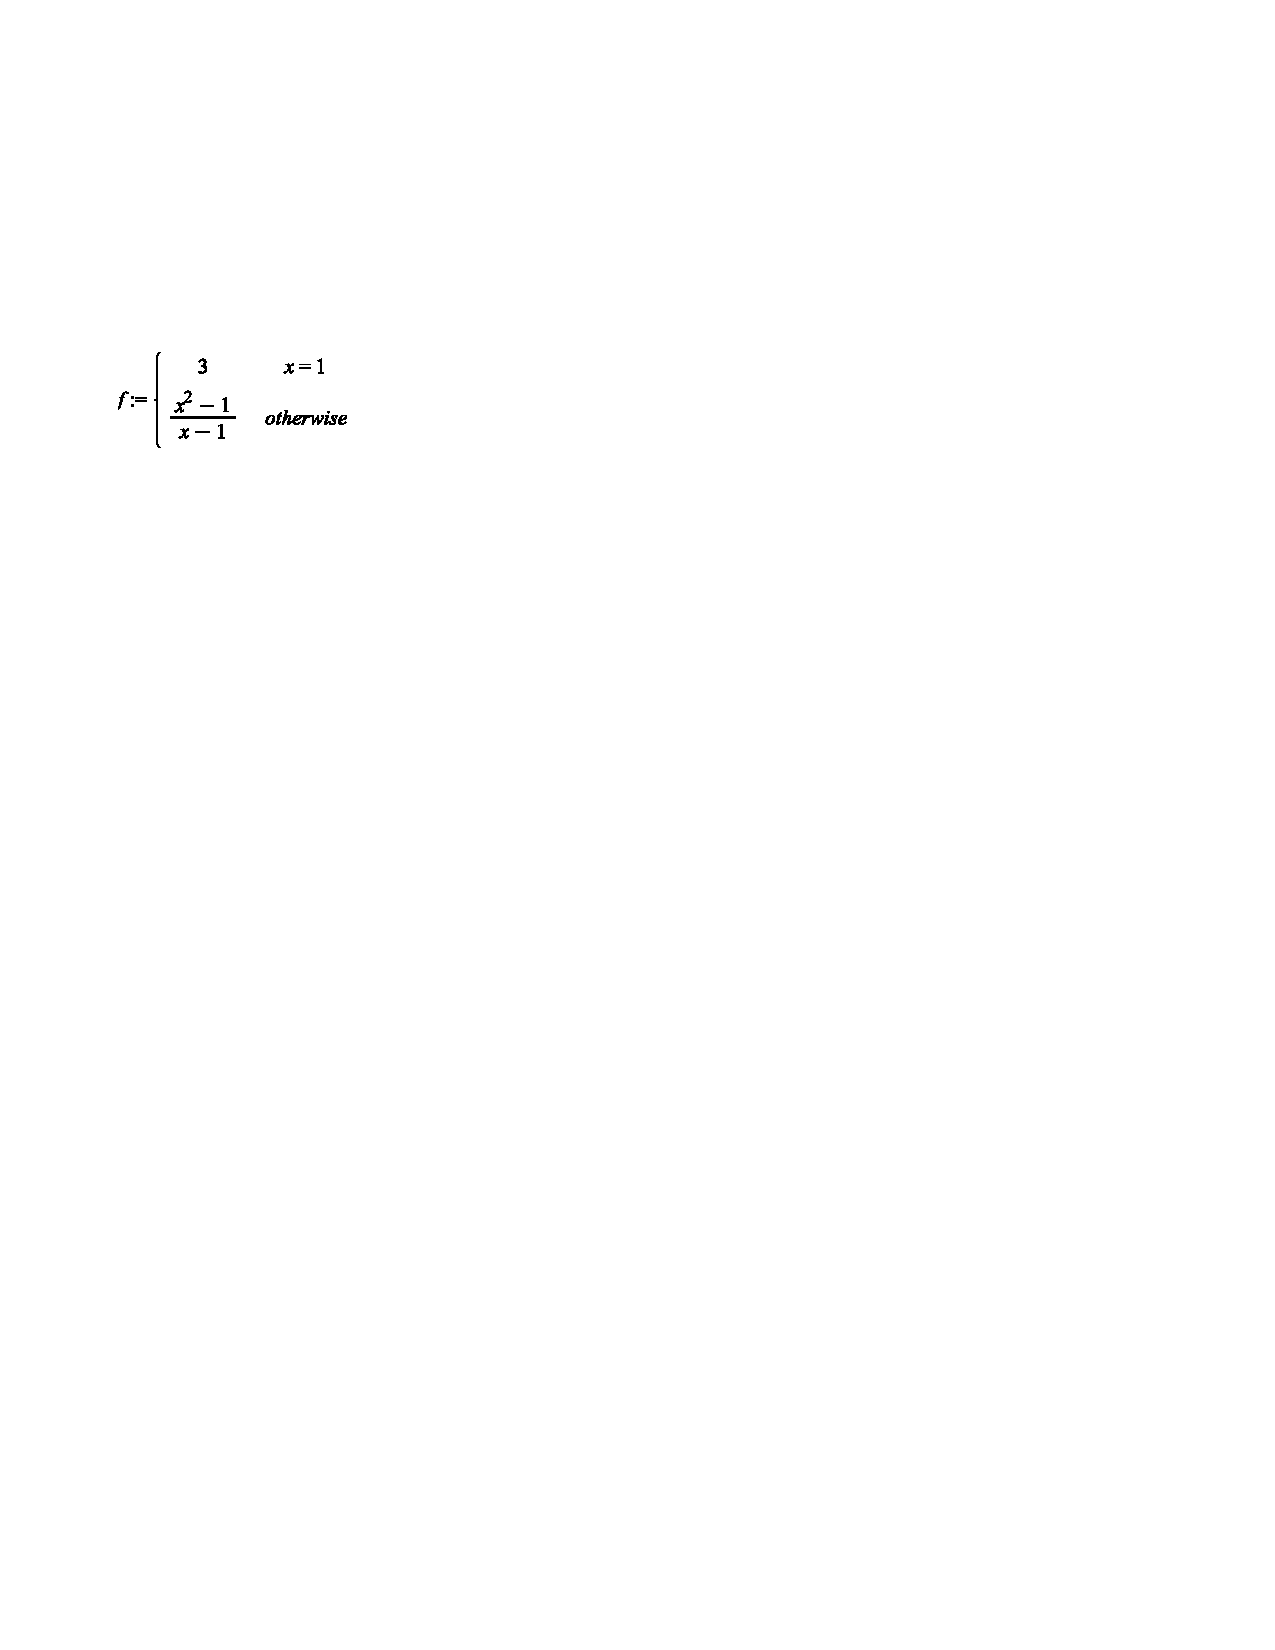
\includegraphics[trim= 70 575 300 165]{Figure7.pdf}
% 			 	\end{image}
			 	
% 			and
			
% 				\begin{image}
% 				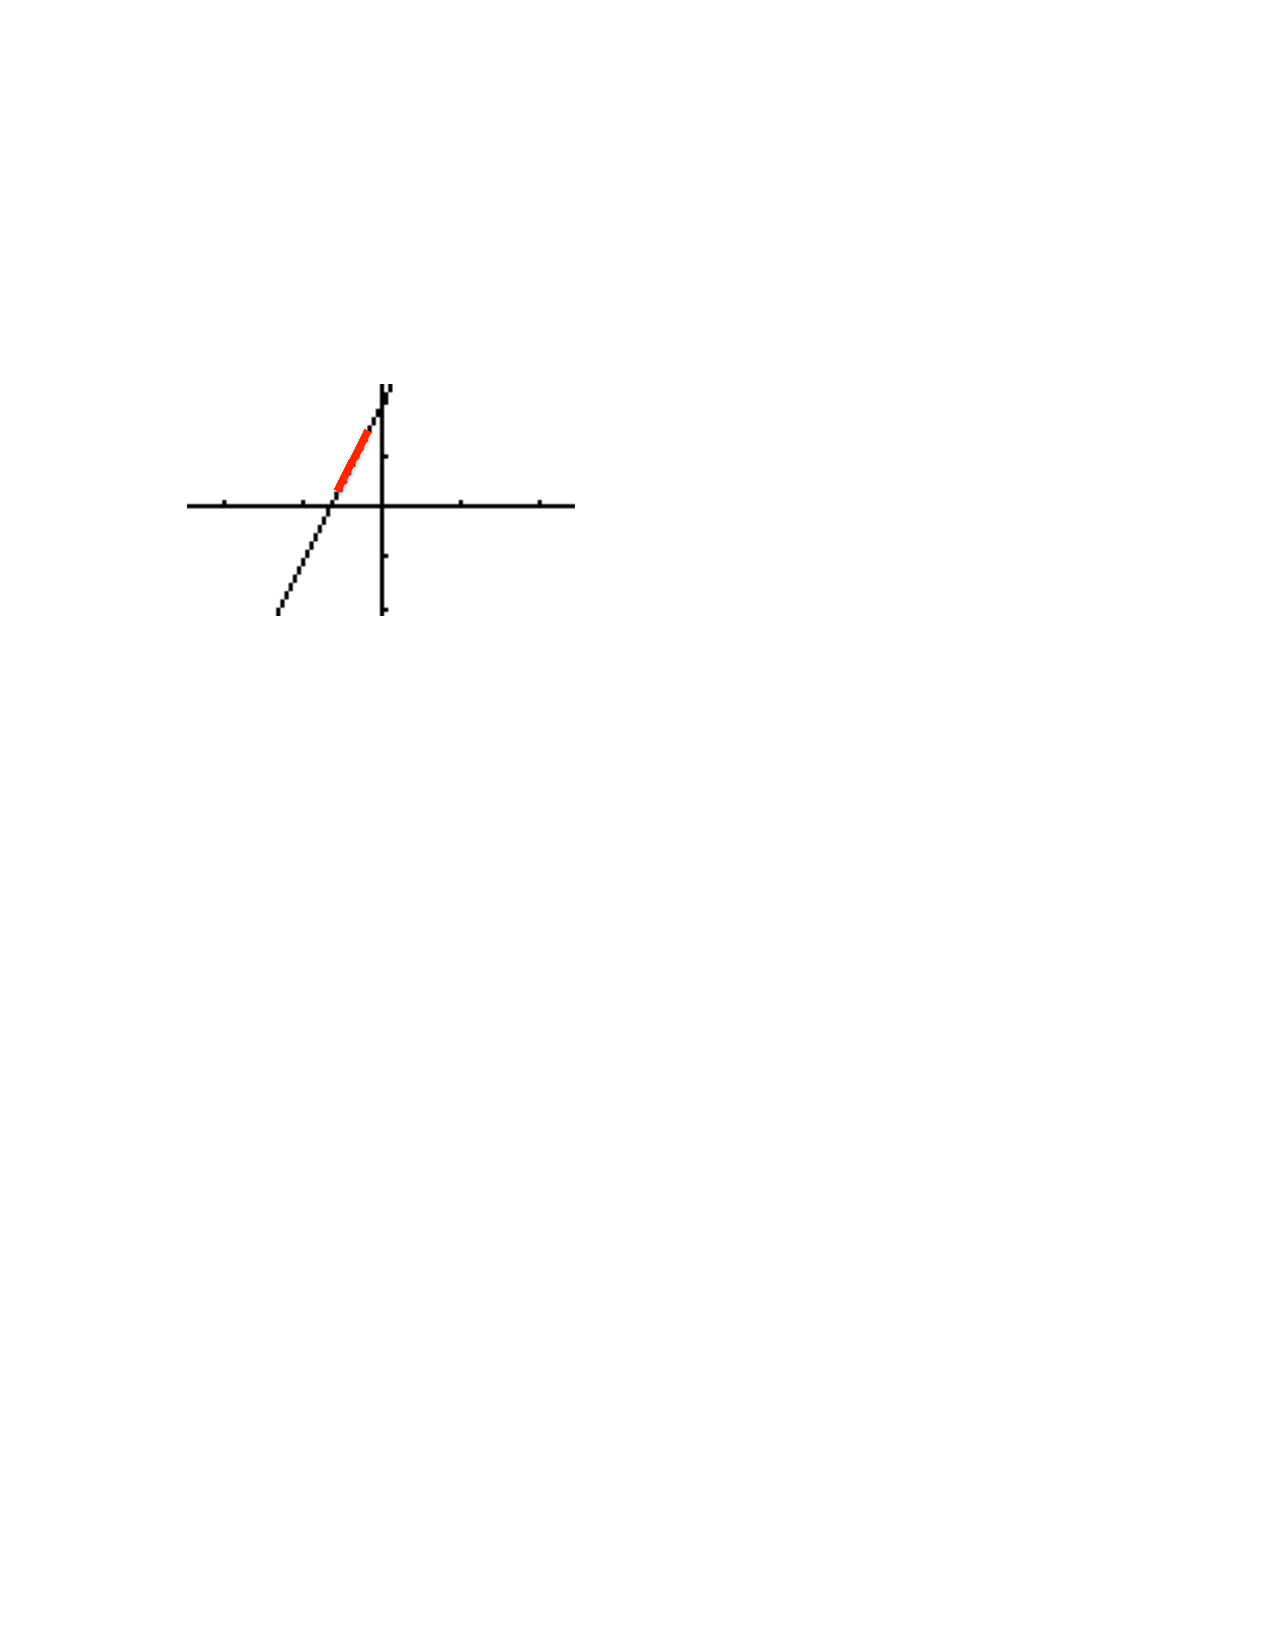
\includegraphics[trim= 70 580 300 165]{Figure8.pdf}
% 				\end{image}
				
% 			 we see that $ \lim_{x \to 1} f(x) = \lim_{x \to 1} g(x) = 2$, but $f(1) = 3$ and $g(1) = 1$.
% 			\end{freeResponse}
			
			
			
% 			%part d
% 			\item  $ \lim_{x \to a} \frac{f(x)}{g(x)} $ does not exist if $g(a) = 0$.
% 			\begin{freeResponse}
% 			False.  If $f(x) = x^3$ and $g(x) = x^2$, then $g(0) = 0$ but $ \lim_{x \to 0} \frac{f(x)}{g(x)} = \lim_{x \to 0} \frac{x^3}{x^2} = \lim_{x \to 0} x = 0$.  
% 			\end{freeResponse}
			
			
			
% 			\end{enumerate}
% \end{problem}
\end{document} 
